\section{Experimental Results}
\label{sec:experimental-results}

	% Overview
	In this section, we present our experimental results. First, we
	analyze outcomes for \textit{Microbenchmarks}, and next we move to a
	discussion on the results for the \textit{Synthetic Benchmarks}. For
	a detailed description about these experiments, see
	Section~\ref{sec:evaluation-methodology}.

\subsection{Microbenchmarks}

	Figure~\ref{fig:lkcall-result} pictures the breakthrough of execution
	time for the \textit{\lkcall Benchmark}. Before proceeding with our
	analysis, it is important to note that hardware events that are
	depicted are not exclusive with each other. For example, an
	\textit{I-Cache Stall} may incur in a \textit{Register Stall}, thus
	the bar labelled \textit{Total Cycles} is not the aggregation of the
	other bars. Noteworthy, this observation applies to the other plots
	that follow.

	\begin{figure}[t]
			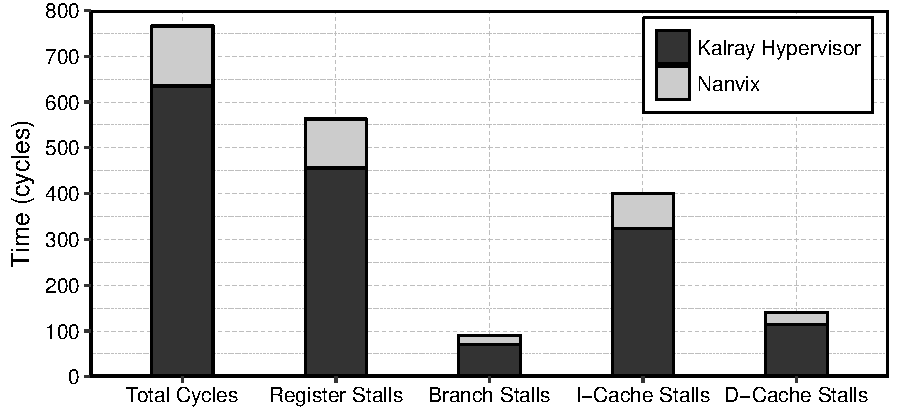
\includegraphics[width=1.00\linewidth]{ukernel-0a0088b/kcall-local-time-breakdown}
			\caption{Execution breakthrough for the \textit{\lkcall Benchmark}.}
			\label{fig:lkcall-result}
	\end{figure}
